\documentclass[10pt,a4paper, margin=1in]{article}
\usepackage{fullpage}
\usepackage{amsfonts, amsmath, pifont}
\usepackage{amsthm}
\usepackage{graphicx}
\usepackage{float}

\usepackage{tkz-euclide}
\usepackage{tikz}
\usepackage{pgfplots}
\pgfplotsset{compat=1.13}

\usepackage{geometry}
 \geometry{
     a4paper,
     total={210mm,297mm},
     left=10mm,
     right=10mm,
     top=10mm,
     bottom=10mm,
 }
 % Write both of your names here. Fill exxxxxxx with your ceng mail address.
 \author{
  Adıgüzel, Gürhan İlhan\\
  \texttt{e2448025@ceng.metu.edu.tr}
  \and
  İçen, Anıl\\
  \texttt{e2448488@ceng.metu.edu.tr}
}

\title{CENG 384 - Signals and Systems for Computer Engineers \\
Spring 2023 \\
Homework 2}
\begin{document}
\maketitle

\begin{filecontents}{q3.dat}
  n  y[n]
 -3  0
 -2  2
 -1  4
  0  1
  1  2
  2  0
  3  0
\end{filecontents}

\noindent\rule{19cm}{1.2pt}

\begin{enumerate}

\item %write the solution of q1
    \begin{enumerate}
    % Write your solutions in the following items.
        \item %write the solution of q1a
        \\\\ $\int x(t) - 5y(t) \,dt = y(t)$
        \\\\
        \item %write the solution of q1b
        \\\\ By getting the differential of the equation above, we get:
        \\\\ \hspace*{50} $y'(t) + 5y(t) = x(t)$
        \\\\ Solving the characteristic equation gives us:
        \\\\ \hspace*{50} $r+5 = 0$
        \\\\ \hspace*{50} $r=-5$
        \\\\ The homogeneous solution is found as $y_{h} = Ke^{-5t}$
        \\\\ We know that the system is linear. Therefore, we can find the particular solutions from:
        \\\\ \hspace*{50} $x(t) = (e^{-t} + e^{-3t})u(t) = e^{-t}u(t) + e^{-3t}u(t)$
        \\\\ \hspace*{50} $x_{1}(t) =e^{-t}u(t) $ and $x_{2}(t) =e^{-3t}u(t)$
        \\\\ We need to find $x_{1} $ and $x_{2}$ After that, we need to add them.
        \\\\ For the first equation:
        \\\\ \hspace*{50} $x_{1}(t) = e^{-t}u(t)$, so $x_{1}(t)$ = 0 for $t<0$ and $e^{-t}$ for $t>0$.
        \\\\ Transfer function for $x_{1}(t)$ is $H(\lambda) = \dfrac{1}{\lambda+5}$. $\lambda = -1$ and $H(-1) = \dfrac{1}{4}$. 
        \\\\ Hence, the particular solution for $x_{1}(t) = \dfrac{1}{4}e^{-t}u(t)$.
        \\\\ We can get the particular solution for $x_{2}(t)$ following the same steps.
        \\\\ \hspace*{50} $x_{2}(t) = e^{-3t}u(t)$ and $H(-3) = \dfrac{1}{2}$
        \\\\ Therefore, particular solution for $x_{2}(t)$ is $\dfrac{1}{2}e^{-3t}u(t)$
        \\\\ \hspace*{50} $y(t) = y_{H}(t) + y_{P}(t) = Ke^{-5t} + \dfrac{1}{4}e^{-t}u(t) +  \dfrac{1}{2}e^{-3t}u(t)$
        \\\\ Finally, we need to find K.
        \\\\ \hspace*{50} $y(0) = K +\dfrac{1}{4}+\dfrac{1}{2} = 0 $
        \\\\ \hspace*{50}  K = $\dfrac{-3}{4}$
        \\\\ Therefore, $y(t) = \dfrac{-3}{4}e^{-5t} + \dfrac{1}{4}e^{-t}u(t) +  \dfrac{1}{2}e^{-3t}u(t)$
    \end{enumerate}

\item %write the solution of q2  
	\begin{enumerate}
    \item %write the solution of q2a
        \begin{align*}
                y[n] &= x[n] * h[n]
                \\ &= \sum_{k=-\infty}^{\infty} x[k] . h[n-k]
                \\ &= \sum_{k=-\infty}^{\infty} (2\delta[k] . \delta[n-k-1] + 2\delta[k+1] . \delta[n-k-1] + \delta[k+1] . 2\delta[n-k+1])
                \\ &= 2 \sum_{k=-\infty}^{\infty} \delta[k] . \delta[n-k-1] + 4 \sum_{k=-\infty}^{\infty} \delta[k] . \delta[n-k+1] +  \sum_{k=-\infty}^{\infty} \delta[k+1] . \delta[n-k-1] + 2 \sum_{k=-\infty}^{\infty} \delta[k+1] . \delta[n-k+1]
                \\\\ &=2.\delta[n-1] + 4.\delta[n+1] + \delta[n] + 2.\delta[n+2]
                \\\\ y[n] &= 2.\delta[n-1] + \delta[n] + 4.\delta[n+1] + 2.\delta[n+2]
        \end{align*}
        \begin{figure}[H]
            \centering
            \begin{tikzpicture}[scale=1.0] 
              \begin{axis}
                [
                  axis lines=middle,
                  xlabel={$n$},
                  ylabel={$y[n]$},
                  xtick={ -3, -2, -1, 0, ..., 3},
                  ytick={0, 1 , 2, 3 , 4},
                  ymin= -1, ymax=5,
                  xmin=-4, xmax=4,
                  every axis x label/.style={at={(ticklabel* cs:1.05)}, anchor=west,},
                  every axis y label/.style={at={(ticklabel* cs:1.05)}, anchor=south,},
                  grid,
                ]
                \addplot [ycomb, black, thick, mark=*] table [x={n}, y={y[n]}] {q3.dat};
              \end{axis}
            \end{tikzpicture}
            \caption{$y[n] = x[n]*h[n]$.}
            \label{fig:q5}
        \end{figure}
        
    \item %write the solution of q2b
        \\\\ $\frac{dx(t)}{dt} = \delta(t-1) + \delta(t+1)$
        \\\\ Since the Convolution is distributive, 
        \begin{align*}
            y(t) &= \dfrac{dx(t)}{dt} * h(t)
            \\ &= h(t) * ( \delta(t-1) + \delta(t+1))
            \\ &= (h(t) *\delta(t-1)) + (h(t) *\delta(t+1))
            \\ &= h(t-1) + h(t+1) 
            \\ y(t) &= e^{-(t-1)}sin(t-1) . u(t-1) + e^{-(t+1)}sin(t+1) . u(t+1)
        \end{align*}
    \end{enumerate}

\item %write the solution of q3
    \begin{enumerate}
        \item %write the solution of q3a
        $y(t) = x(t)h(t) = \int_{-\infty}^{\infty}e^{-\tau}u(\tau)e^{-2(t-\tau)}u(t-\tau)d\tau$
        \\\\ Since $u(\tau)$ and $u(t-\tau)$ does not overlap when $t<0$, we do not need to consider that interval.
        \\\\ But, we need to consider when $t>0$, because they overlap in that interval. 
        \\\\ So, we need to change the limits of the integral in the interval 0 to t.
        \\\\ $y(t) = \int_{0}^{t}e^{-t}e^{-2(t-\tau)}\,d\tau$
        \\\\ $= e^{-2t} \int_{0}^{t}e^{\tau}\,d\tau$
        \\\\ $=e^{-2t}(e^{t} -1)$
        \\\\ $=(e^{-t} - e^{-2t})u(t)$
        \\
        \item %write the solution of q3b
        \\$x(t) = u(t) - u(t-1)$
        \\\\ $ = \delta(t-1)$
        \\\\ $y(t) = x(t) * h(t)$
        \\\\ $= \delta(t-1) * h(t)$
        \\\\ $= h(t-1)$
        \\\\ $y(t) = e^{3(t-1)} . u(t-1)$
        \\\\
    \end{enumerate}

\item %write the solution of q4
    \begin{enumerate}   
        \item %write the solution of q4a
        $y[n] - y[n-1] - y[n-2] = 0, y[0]=1$ and $y[1]=1$
        \\\\ $r^2 - r -1 = 0$
        \\\\ $r_{1} = \dfrac{1+\sqrt5}{2}$
        \\\\ $r_{2} = \dfrac{1-\sqrt5}{2} $
        \\\\ $y[n] = A (\dfrac{1+\sqrt5}{2})^n + B(\dfrac{1-\sqrt5}{2})^n $
        \\\\ $y[0] = A + B = 1$
        \\\\ $y[1] = A \dfrac{1+\sqrt5}{2} + B\dfrac{1-\sqrt5}{2} = 1$
        \\\\ $y[1] - \dfrac{y[0]}{2} = \dfrac{\sqrt{5}}{2}(A-B) = \dfrac{1}{2} $
        \\\\ $A-B = \dfrac{1}{\sqrt{5}}$
        \\\\ $A+B = 1$
        \\\\ $A = \dfrac{1+\dfrac{1}{\sqrt{5}}}{2} = \dfrac{\sqrt{5}+1}{2\sqrt{5}}$
        \\\\ $B = \dfrac{1-\dfrac{1}{\sqrt{5}}}{2} = \dfrac{\sqrt{5}-1}{2\sqrt{5}}$
        \\\\ Therefore: 
        \\\\ $y[n] =  \dfrac{\sqrt{5}+1}{2\sqrt{5}} (\dfrac{1+\sqrt(5)}{2})^n +  \dfrac{\sqrt{5}-1}{2\sqrt{5}}(\dfrac{1-\sqrt(5)}{2})^n$
        \\
        \item %write the solution of q4b
        \\\\$y^(3)(t) - 6y''(t) + 13y'(t) - 10y(t) = 0, y''(0) =3, y'(0) =\dfrac{3}{2} and, y(0) = 1.$
        \\\\$r^3 - 6r^2 +13r+ 10 = 0$
        \\\\$ = (r-2) (r - (2+j))(r - (2-j))$
        \\\\$y(t) = Ae^{2t} + Be^{(2+j)t}+Ce^{(2-j)t$
        \\\\$y(0) = A+B+C = 1$
        \\\\$y'(0) = 2A + (2+j)B + (2-j)C = \dfrac{3}{2}$
        \\\\$= 2(A+B+C) + j(B-C)$
        \\\\$j(B-C) = \dfrac{-1}{2}$
        \\\\$y''(0) = 4A + (2+j)^{2}B + (2-j)^{2}C = 3$
        \\\\$= 4A+3B+3C+4j(B-C)$
        \\\\$A + 4j(B-C) = 0$
        \\\\$A = 2$
        \\\\$B+C = -1$
        \\\\$B-C = \dfrac{j}{2}$
        \\\\$B = \dfrac{j-2}{4} C = \dfrac{-j-2}{4}$
        \\\\$y(t) = 2e^{2t} + \dfrac{j-2}{4}e^{(2+j)t} +  \dfrac{-j-2}{4}e^{(2-j)t}$
        \\\\ $= e^{2t}(2 + \dfrac{j-2}{4}(cos(t)+jsin(t)) + \dfrac{-j-2}{4}(cos(t)-jsin(t))) $
        \\\\ $y(t) = e^{2t}[2 - \dfrac{1}{2}(sin(t)+2cos(t))]$
        \\\\
    \end{enumerate}

\item %write the solution of q5
    \begin{enumerate}
        \item %write the solution of q5a
        \\\\ $y_p(t) = Kx(t) = Kcos(5t)$
        \\\\\ K = $ H(\lambda) = \dfrac{\sum_{k=0}^{M}{b_k \lambda^{k}}}{\sum_{k=0}^{N}{a_k \lambda^{k}}}$
        \\\\ According to the Euler's formula :
        \\\\ $cos(5t) = \dfrac{(e^{j5t} + e^{-j5t})}{2}$
        \\\\ $y_p(t) = Kcos(5t) = \dfrac{K.e^{j5t} + K.e^{-j5t}}{2}$
        %\\\\ $sin(5t) = \dfrac{(e^{j5t} - e^{-j5t})}{2j}$
        \\\\ For $x_1(t) = e^{j5t}, \lambda $ is $(j5t)$, so using the formula of the Transfer function:
        \\\\ We have $H(j5) = \dfrac{j5}{(j5)^2 + 5(j5) + 6}$
        \\\\ For $x_1(t),$ the particular solution is $H(j5)e^{j5t}$ 
        \\\\ For $x_2(t),$ the particular solution is $H(-j5)e^{-j5t}$
        \\\\ For $x(t) = \dfrac{x_1(t) + x_2(t)}{2},$ the particular solution is:
        \\\\ $y_p(t) = \dfrac{H(j5)e^{j5t} + H(-j5)e^{-j5t}}{2}$
        \\
        \item %write the solution of q5b
        \\\\ Assume $y_h(t) = Ce^{st} $  $ => $  $ Cs^{2}e^{st} + 5Cse^{st} + 6Ce^{st} = \emptyset $
        \\\\ $y_h(t) = C (s^{2} + 5s + 6)e^{st} $
        \\\\ So, (S = -3) or (S = -2)
        \\\\ $y_h(t) = C_1e^{-3t} +  C_2e^{-2t} $
        \\
    	\item %write the solution of q5c
        \\\\ $y(t) = y_h(t) + y_p(t)$
        \\\\ Use initially at rest condition is $y(0) = 0 $ and $ y'(0) = 0$
        \\\\ $y(0) = y_h(0) + y_p(0) = 0$
        \\\\ $y(0) =  C_1e^{-3.0} +  C_2e^{-2.0} + \dfrac{H(j.5)e^{j.5.0} + H(-j.5)e^{-j.5.0}}{2} = 0$
        \\\\ $C_1 + C_2 + \dfrac{H(5j)}{2} + \dfrac{H(-5j)}{2} = 0$
        \\\\ $ H(5j) = \dfrac{5j}{25j-19} $ \hspace*{10} and \hspace*{10} $ H(-5j) = \dfrac{-5j}{-25j-19}$
        \\\\\\ $C_1 + C_2 = \dfrac{5j.(25j+19) + 5j(25j-19)}{-(25^2 + 19^2) . 2}$
        \\\\\\ $C_1 + C_2 = \dfrac{-250}{-986 . 2} = \dfrac{125}{986}$
        \\\\ $y'(0) =  -3C_1e^{-3.0} +  -2C_2e^{-2.0} + \dfrac{(5j)H(j.5)e^{j.5.0} + (-5j)H(-j.5)e^{-j.5.0}}{2} = 0$
        \\\\\\ $-3C_1 + -2C_2 + \dfrac{(5j)H(5j)}{2} + \dfrac{(-5j)H(-5j)}{2} = 0$
        \\\\\\ $ (5j).H(5j) = \dfrac{-25}{25j-19} $ \hspace*{10} and \hspace*{10} $ (-5j).H(-5j) = \dfrac{25}{-25j-19}$
        \\\\\\ $3C_1 + 2C_2 = \dfrac{-950}{-986.2} = \dfrac{475}{986}$
        \\\\\\ $C_1 = \dfrac{225}{986}$ \hspace*{10} and \hspace*{10} $C_2 = \dfrac{-100}{986}$
        \\\\ $y(t) = (\frac{225}{986})e^{-3t} + (\frac{-100}{986})e^{-2t} + \dfrac{H(j.5)e^{j.5.t} + H(-j.5)e^{-j.5.t}}{2}$
        \\\\
    \end{enumerate}    
    
\item %write the solution of q6
    \begin{enumerate}
        \item %write the solution of q6a
        $h_0[n] - \dfrac{1}{2}h_0[n-1] = \delta[n] \rightarrow h_0[n] = \dfrac{1}{2}h_0[n-1] + \delta[n]$
        \\\\ If the system is initially at rest:
        \\\\ $h_0[n] = 0$ for all $ n<0$.
        \\\\ $h_0[n] = \dfrac{1}{2}h_{0}[n-1] + \delta[0] = 0+1 = 1$
        \\\\ $\delta[n] = 0 $ for all $ n>0.$ Thus for $n>0$,
        \\\\ $h_0[n] =\dfrac{1}{2^{n}} . u[n]$
        \\
        \item %write the solution of q6b
        \\\\ $h[n] = h_0[n] . h_0[n] = \sum_{k=-\infty}^{\infty} \dfrac{1}{2^{k}} . u[k] . \dfrac{1}{2^{n-k} . u[n-k]}$
        \\\\ If $n<0$ and $u[n-k]$ do not overlap, then $h[n] = 0$.
        \\\\ If $n\geq 0$ and $ 0 \geq u[n-k] \geq n$, then Limits of the Sum can be changed.
        \\\\ $h[n] = \sum_{k=0}^{n} \dfrac{1}{2^{k}} . \dfrac{1}{2^{n-k}} =  \sum_{k=0}^{n} \dfrac{1}{2^{n}} = \dfrac{n}{2^{n}}$
        \\\\ As a result, $h[n] = \dfrac{n}{2^{n}} . u[n]$
        \\
    	\item %write the solution of q6c
        $ w[n] = y[n] - \dfrac{y[n-1}{2}]$
        \\\\ Since the System is the LTI system:
        \\\\ $\dfrac{y[n-1]}{2} - \dfrac{y[n-2]}{4} = \dfrac{w[n-1]}{2}$
        \\\\ We have two equations now. When we subtract them from each other, 
        \\\\ $x[n] = y[n] - y[n-1] + \dfrac{y[n-2]}{4} = w[n] - \dfrac{w[n-1]}{2}$
        \\\\ $x[n] = y[n] - y[n-1] + \dfrac{y[n-2]}{4}$
        
    \end{enumerate}
 \newpage   
\item %write the solution of q7
    \begin{enumerate}
        \begin{verbatim}
                import matplotlib.pyplot as plt
                import numpy as np
                
                def convolution(signal1, start1, signal2, start2):
                    len_x = len(signal1)
                    len_h = len(signal2)
                    len_y = len_x+len_h+1
                    y = np.zeros(len_y)
                    for n in range(len_y):
                        for k in range(len_x):
                            if n - k >= 0 and n - k < len_h:
                                y[n] += signal1[k] * signal2[n - k]
                
                    return y
                
                
                filename = "hw2_signal.csv"
                data = np.loadtxt(filename, delimiter=",")
                startIndex = int(data[0])
                signalList = data[1:]
                N = 20  # will change
                h = []
                len_x = len(signalList)
                for i in range(0, len_x):
                    if (0 <= i+startIndex and i+startIndex <= N-1):
                        h.append(1/N)
                    else:
                        h.append(0)
                lst = convolution(signalList, startIndex, h, startIndex)
                n = np.arange(startIndex, startIndex+len(signalList)*2+1)
                
                plt.stem(n, lst, linefmt='b-', markerfmt='bo', label="y[n]")
                plt.legend()
                plt.show()
            \end{verbatim}

        %\item write the solution of q7a
         a) The effect of convolution with $\delta[n-5]$ is shifting the signal to the right by 5.
            \begin{figure}[htp] \centering{
                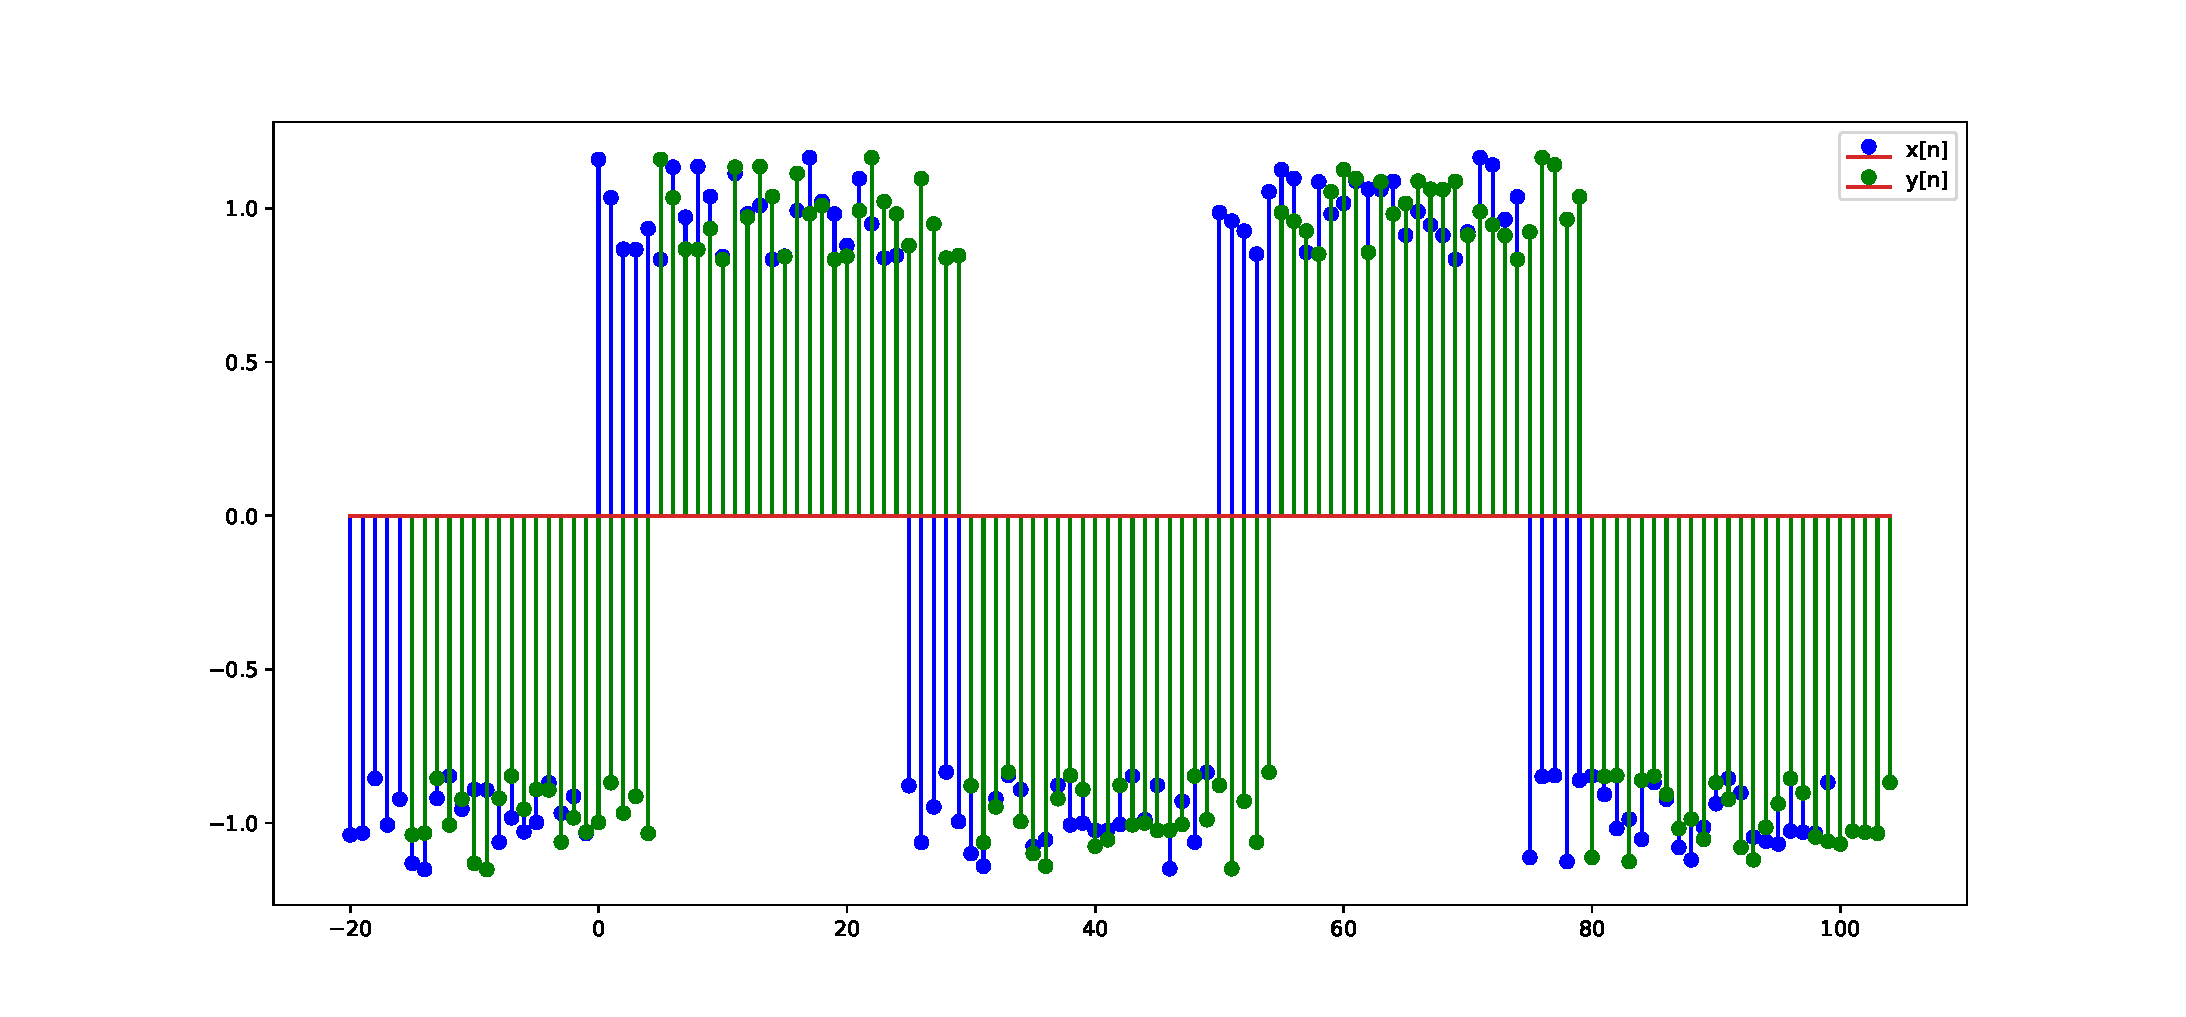
\includegraphics[scale=0.55]{hw2_7a.pdf}}
                \caption{y[n]}
            \end{figure}
        
        %\item %write the solution of q7b
        \newpage
        b) The effect of m[n] is that it produces a smoothed version of the input signal by averaging adjacent samples. The smoothing effect is more prominent as the length of the filter N increases.

        \\The differences between different N values are that a larger N will result in a smoother output signal with more attenuation of high-frequency components.
            \begin{figure}[htp] \centering{
                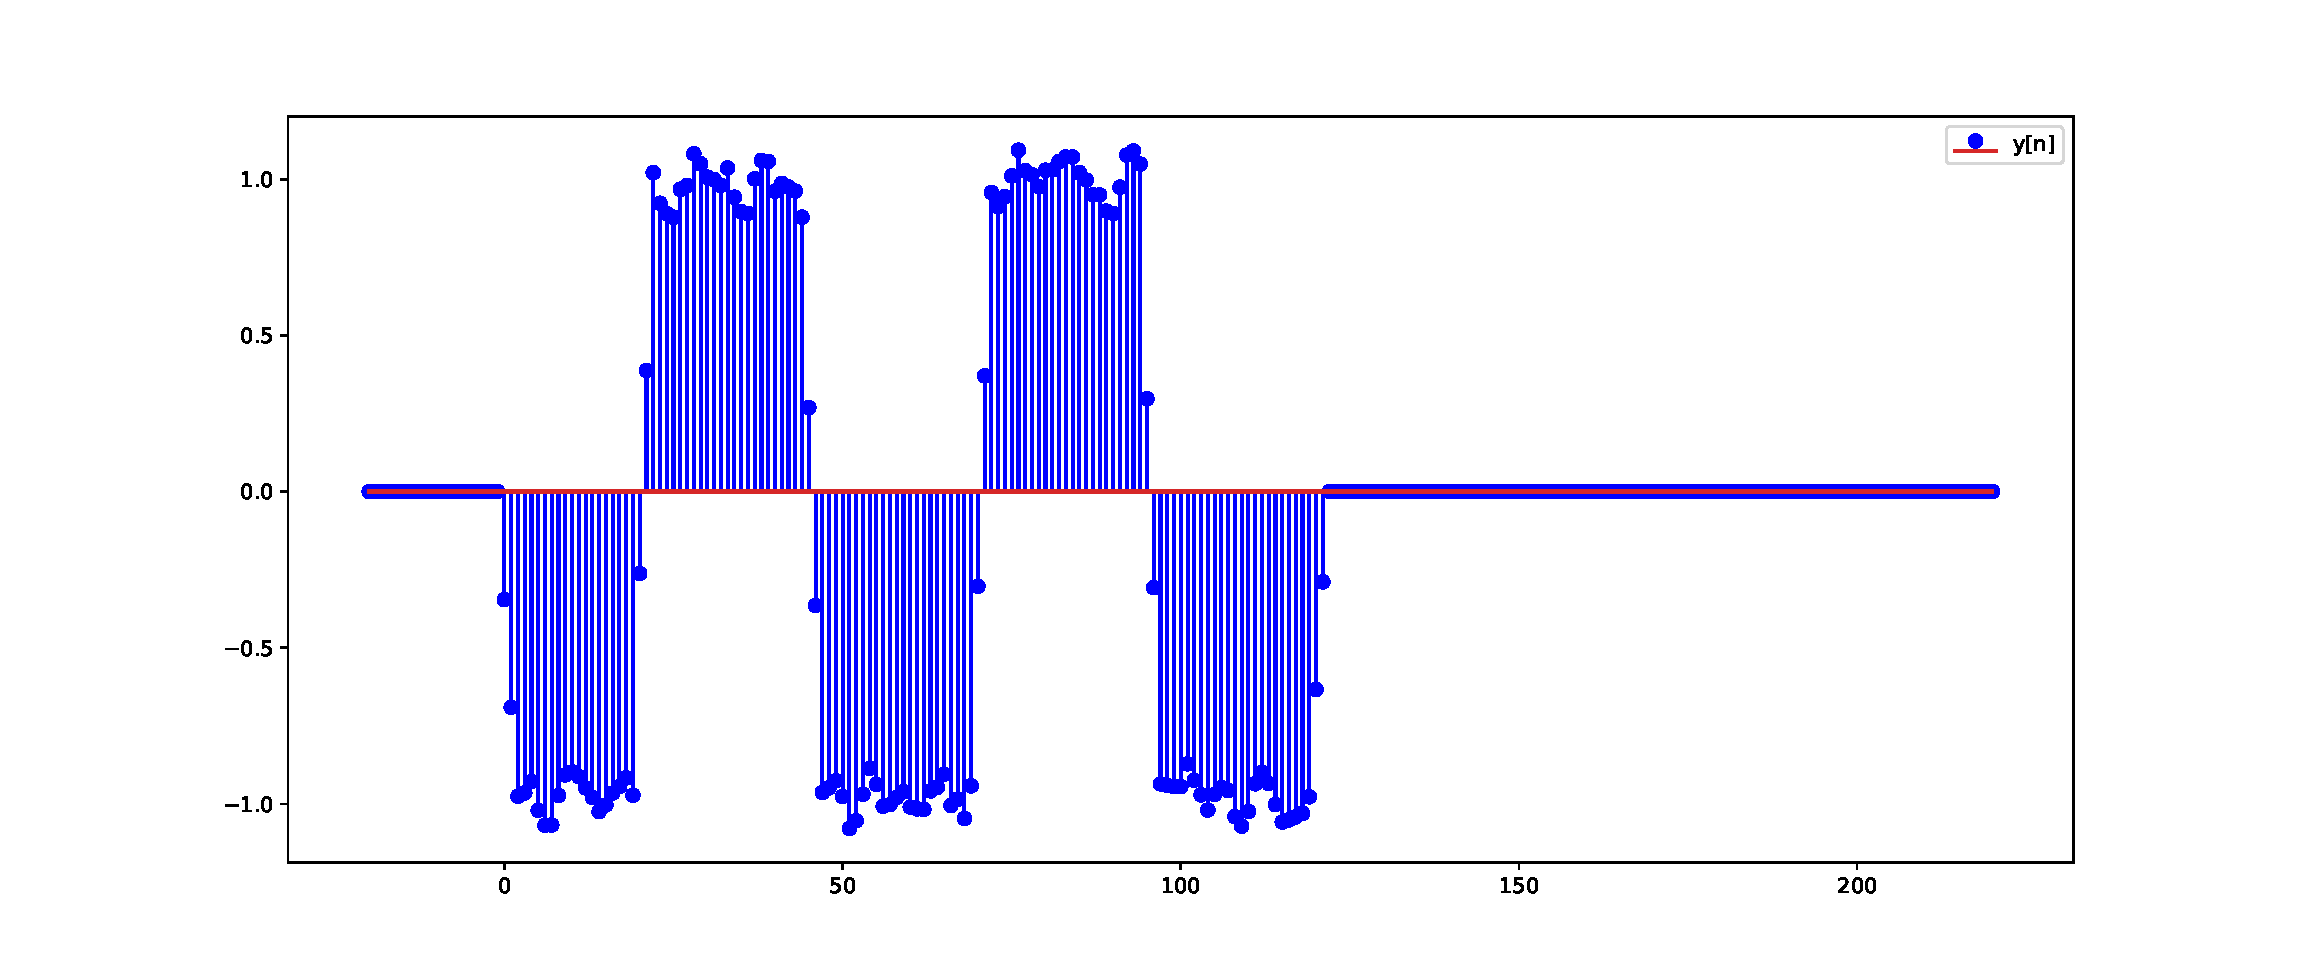
\includegraphics[scale=0.55]{hw2_7b_n3.pdf}}
                \caption{N=3}
            \end{figure}
            \begin{figure}[htp] \centering{
                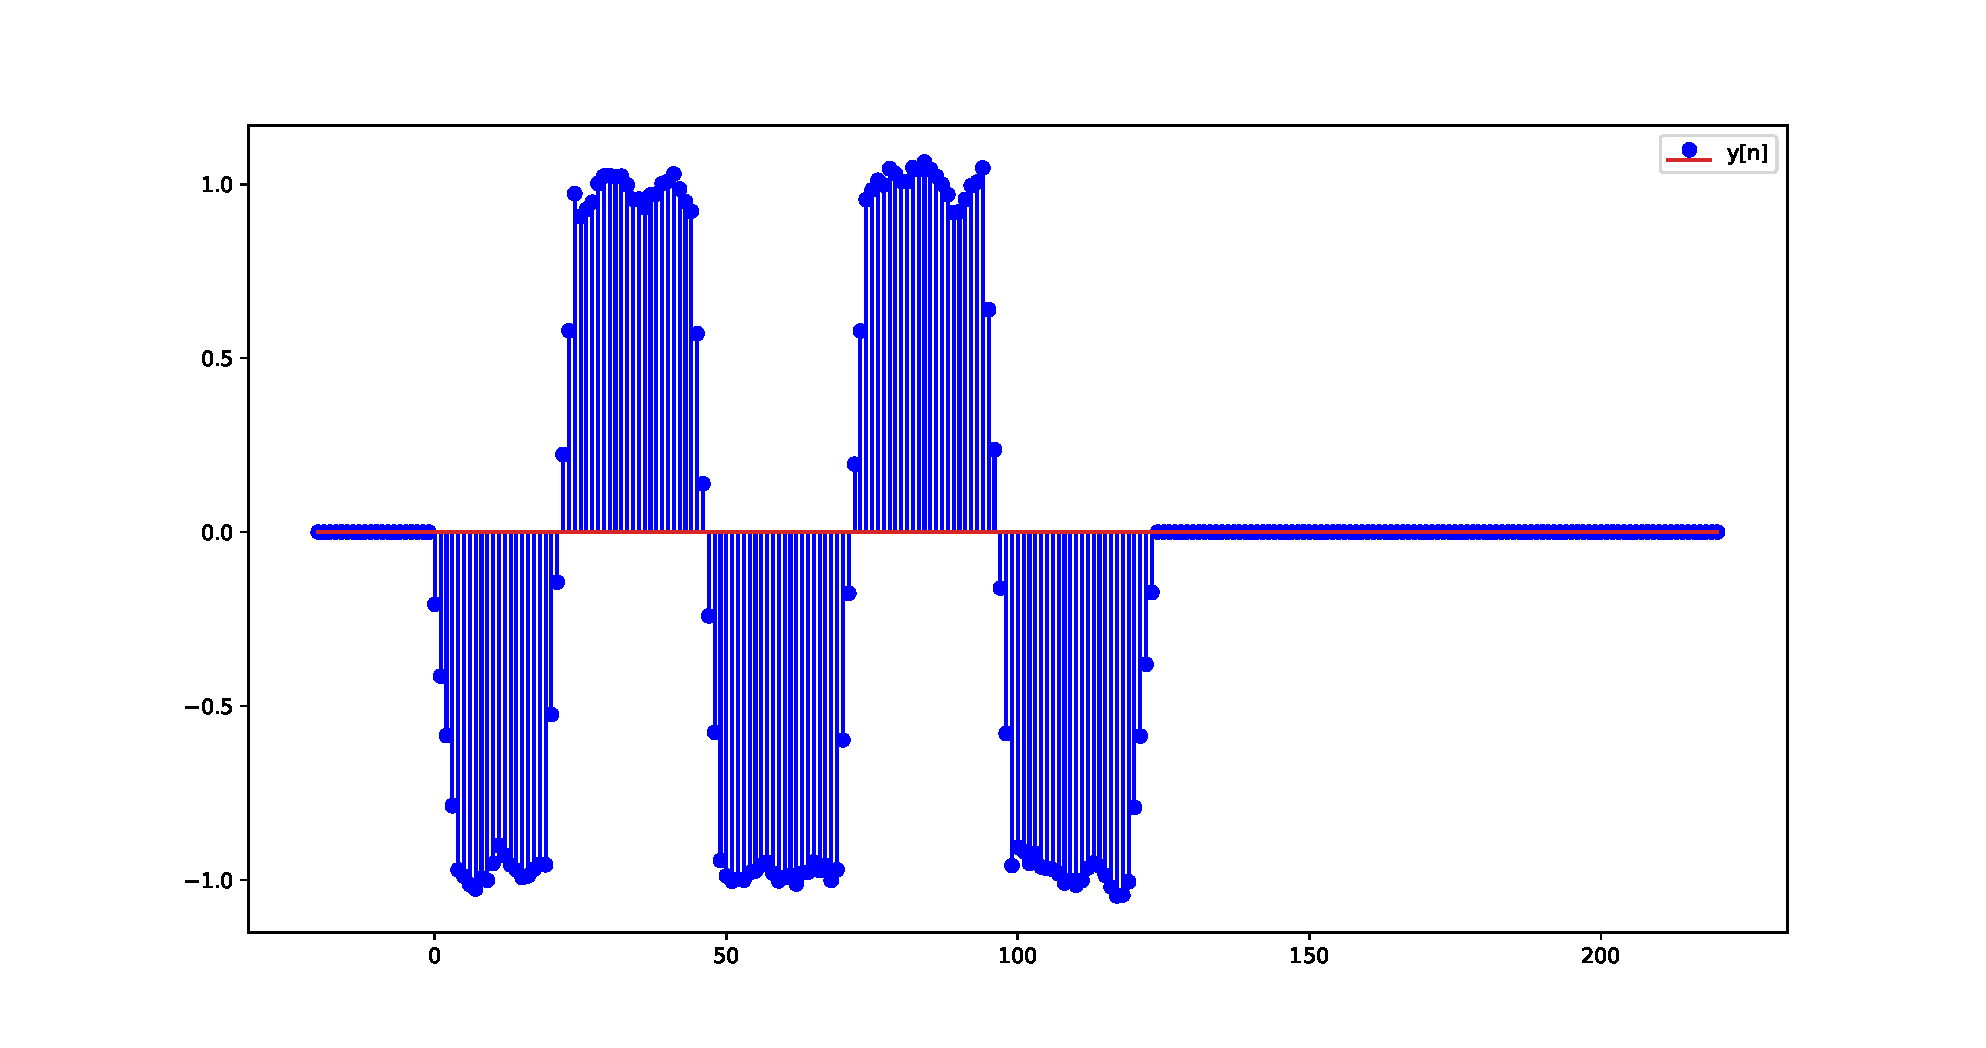
\includegraphics[scale=0.55]{hw2_7b_n5.pdf}}
                \caption{N=5}
            \end{figure}
            \begin{figure}[htp] \centering{
                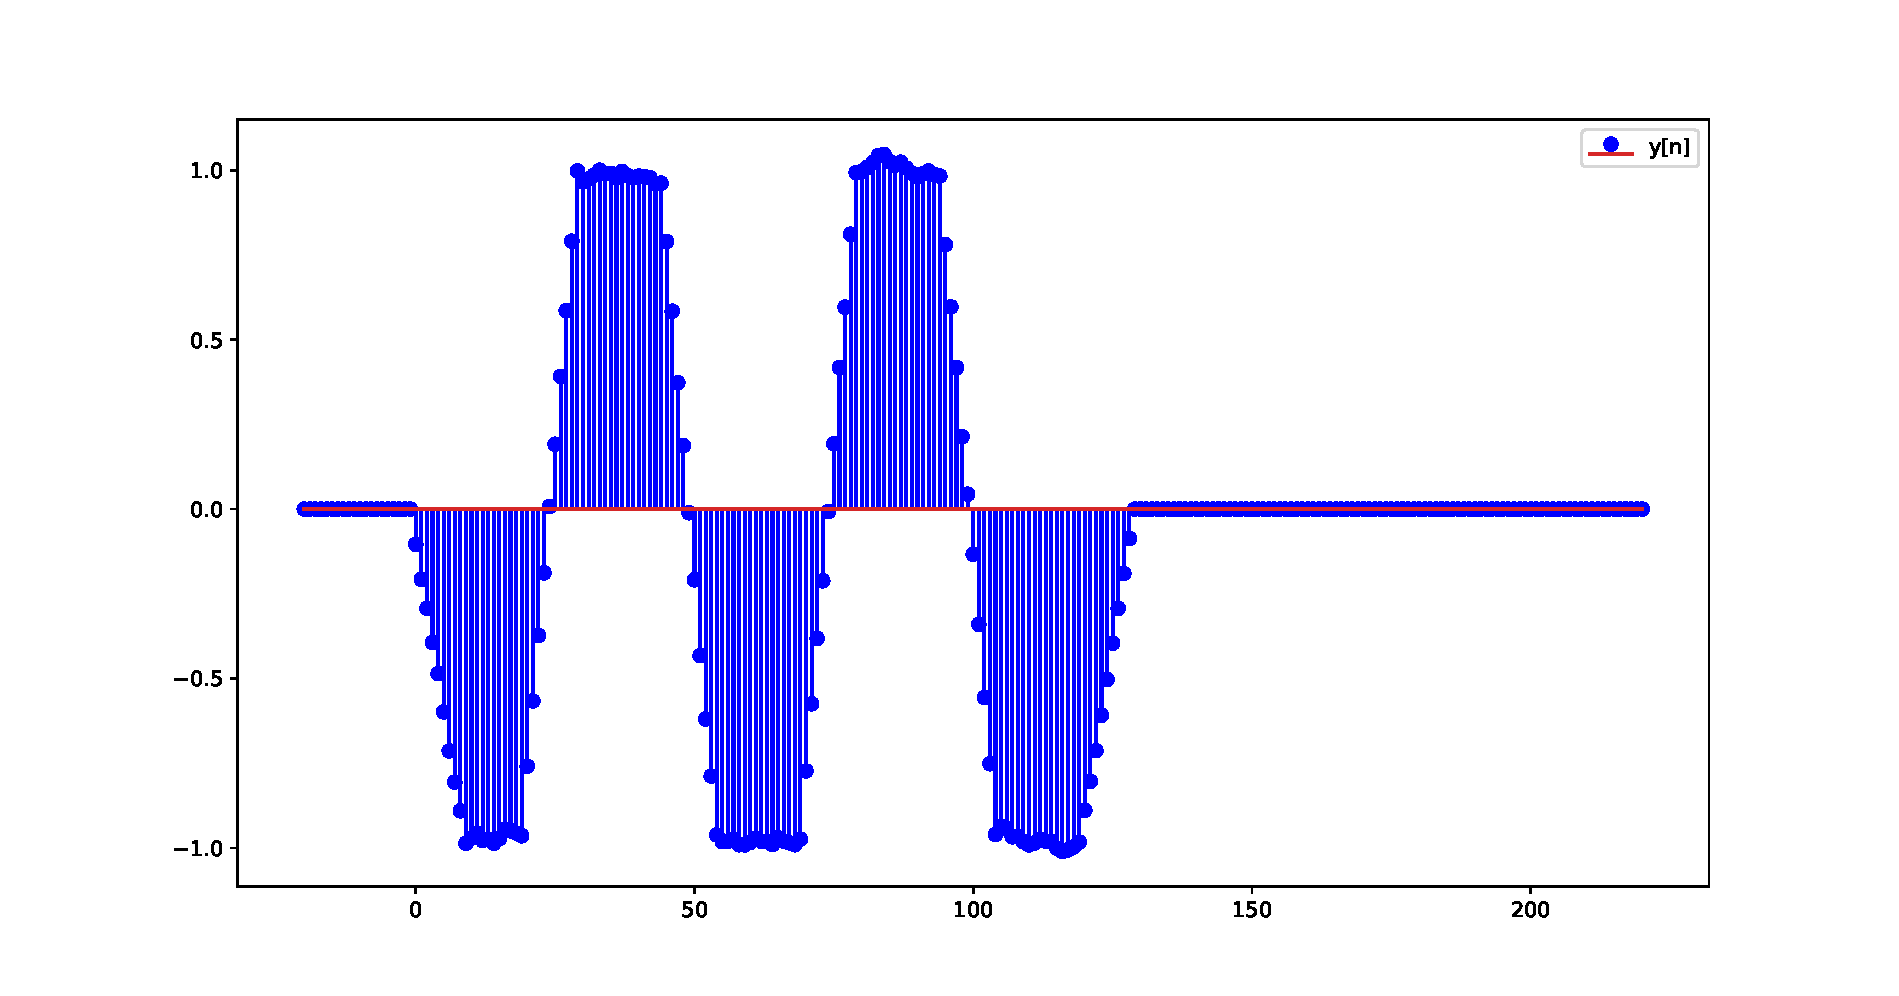
\includegraphics[scale=0.55]{hw2_7b_n10.pdf}}
                \caption{N=10}
            \end{figure}
            \begin{figure}[htp] \centering{
                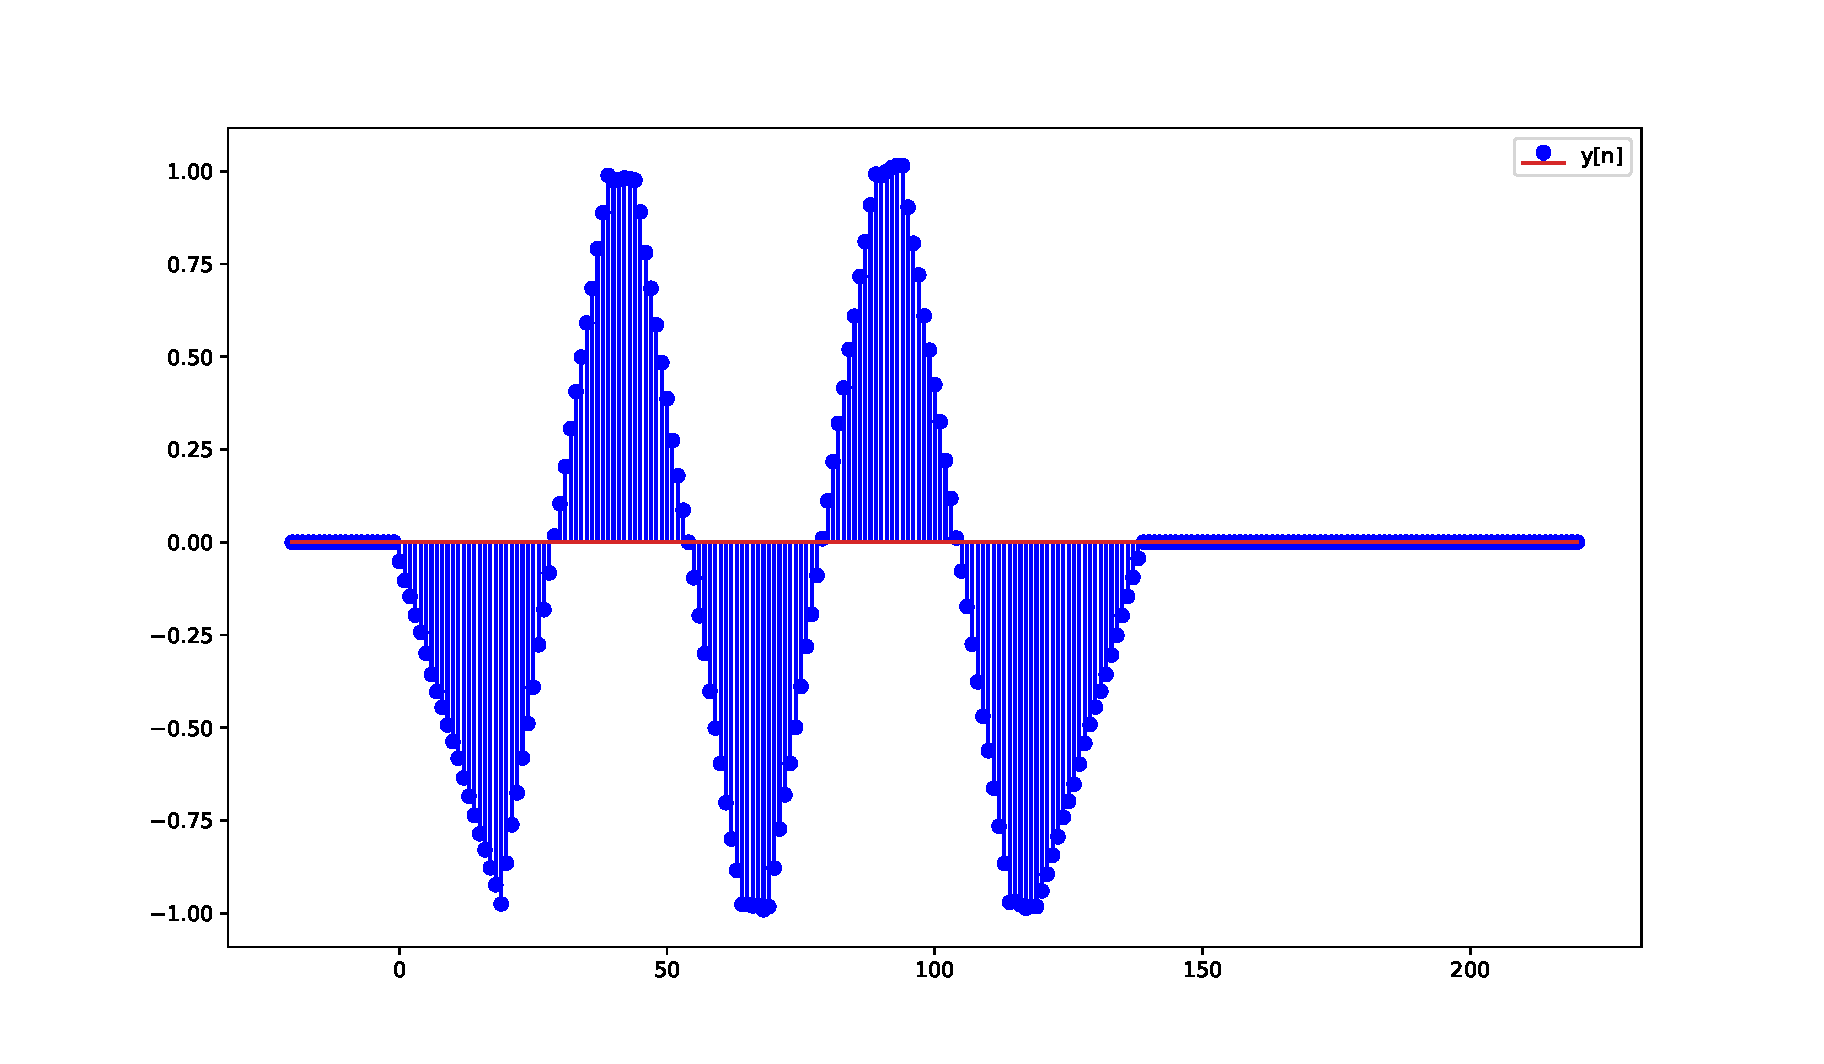
\includegraphics[scale=0.55]{hw2_7b_n20.pdf}}
                \caption{N=20}
            \end{figure}
    \end{enumerate}    
\end{enumerate}
\end{document}

